\begin{boiboiboite}
	\propeau
\end{boiboiboite}

\subsubsection{Température et pression d’ébullition}

	Un/e étudiant/e voyage à bord d’un avion de ligne et se voit servir une boisson chaude (\cref{fig_cafe}) par l’équipage ; la boisson est presque à ébullition. Il/elle en mesure la température à~\SI{88,2}{\degreeCelsius}.	
	
	\begin{enumerate}
		\item Quelle est la pression dans la cabine ?
	\end{enumerate}
	
	L’avion subit une dépressurisation rapide et la pression de la cabine s’égalise avec la pression atmosphérique locale (\SI{17,2}{\kilo\pascal}). L’étudiant/e enfile son masque à oxygène et constate avec déplaisir que la boisson, qui refroidit, s’est mise à bouillir. 
	
	\begin{enumerate}
	\shift{1}
		\item À quelle température l’ébullition cessera-t-elle ?
	\end{enumerate}
	
	\begin{figure}[htp] %handmade
		\begin{center}
			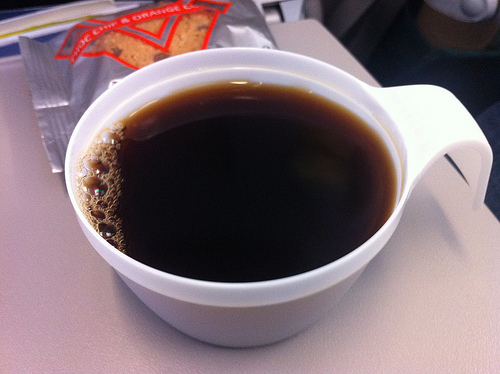
\includegraphics[width=5cm]{images/exercice_cafe.jpg}
		\end{center}
		\supercaption{Boisson chaude aérienne au goût non identifié.}{\href{https://secure.flickr.com/photos/notbrucelee/7942977960/}{photo} \ccby par \flickru{notbrucelee}}
		\label{fig_cafe}
	\end{figure}

\subsubsection{Évaporation d’eau}

	\begin{enumerate}
		\item Combien faut-il de chaleur pour évaporer entièrement une casserole d’eau ? Le récipient contient \SI{2.5}{\liter} d’eau à~\SI{10}{\degreeCelsius}, et la pression atmosphérique ambiante est de~\SI{1}{\bar}. 
		\item Représentez qualitativement l’évolution de l’eau sur un diagramme température-volume (en y représentant la courbe de saturation).
		\item Le réchauffement est effectué avec une plaque électrique de~\SI{1500}{\watt}. Combien de temps faut-il pour vaporiser l’eau, et quel est le coût engendré par l’expérience ? L’opérateur facture \num{0,15}\euro{} par \si{\kilo\watt\hour} et les pertes de la plaque dans la pièce sont de l’ordre de~\SI{10}{\percent}. 
	\end{enumerate}

	\begin{figure}[htp] %handmade
		\begin{center}
			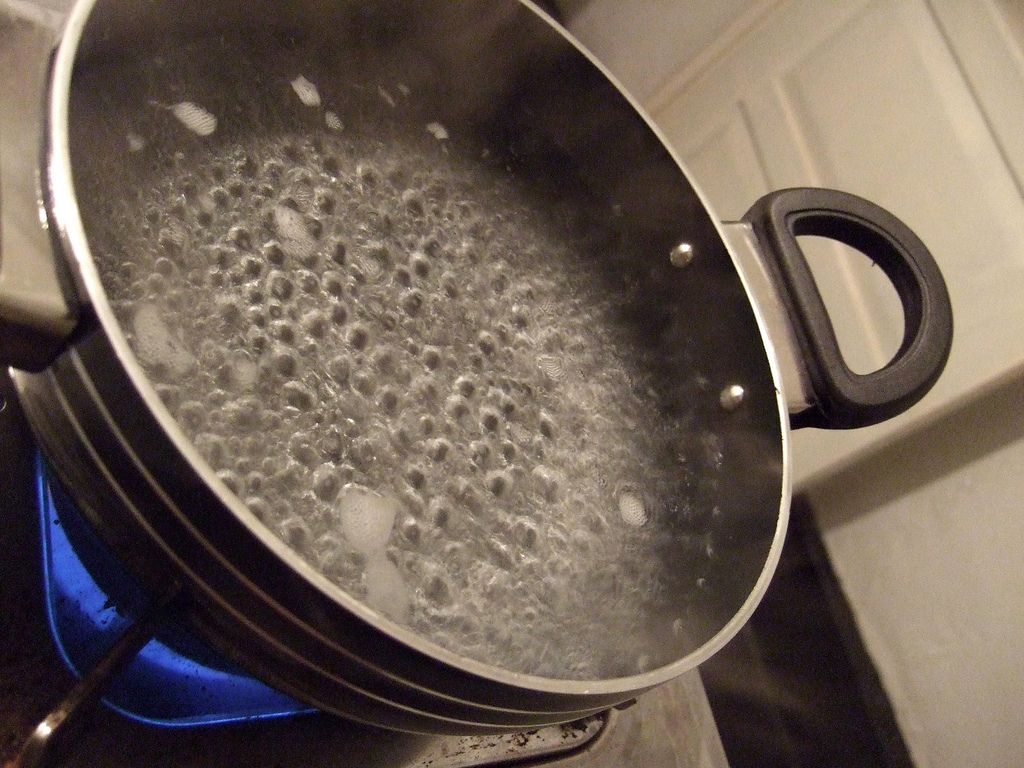
\includegraphics[width=8cm]{images/exercice_boiling.jpg}
		\end{center}
		\supercaption{Expérience de physique ordinaire}{photo \ccby par \flickrun{indi}{Indi Samarajiva}}
	\end{figure}

\subsubsection{Exercice simple de cours}

	\begin{samepage}
	Décrivez très brièvement une expérience permettant de réchauffer à température constante une masse fixe d’eau liquide sous-refroidie. Représentez qualitativement l’évolution sur un diagramme pression-volume (en y représentant la courbe de saturation).
	\end{samepage} %handmade


\subsubsection{Génération de vapeur à haute pression}

	Un procédé industriel chimique nécessite l’apport d’un débit de vapeur de~\SI{2}{\kilogram\per\second} à~\SI{6}{\bar} et~\SI{875}{\degreeCelsius}. La machine en charge de fournir cette vapeur est alimentée par une canalisation d’eau liquide pressurisée à~\SI{10}{\degreeCelsius} et~\SI{6}{\bar}.

	\begin{enumerate}
		\item Quelles puissances sous forme de travail et de chaleur sont nécessaires pour générer ce débit ?
		\item Tracez qualitativement l’évolution subie par l’eau sur un diagramme température-volume.
	\end{enumerate}


\subsubsection{Tout est dans le bouchon}

	Un/e étudiant/e décide de maintenir une alimentation équilibrée, et fait cuire des aliments dans un autocuiseur (couramment appelé «~cocotte-minute~», \cref{fig_cocotte}). 
		
	La soupape (couramment appelée «~bouchon~») de l’autocuiseur pèse \SI{216}{\gram} ; elle est posée sur un conduit d’échappement de diamètre \SI{5}{\milli\metre}. La pression atmosphérique ambiante est de~\SI{1,1}{\bar}.
	
	\begin{enumerate}
		\item À quelle température l’autocuiseur permet-il de faire cuire les aliments ?
		\item Quelle température et quelle pression une personne pourrait-elle générer à l’intérieur de l’autocuiseur en appuyant sur la soupape ? Comment empêcher un accident ?
	\end{enumerate}

	\begin{figure}[htp] %handmade
		\begin{center}
			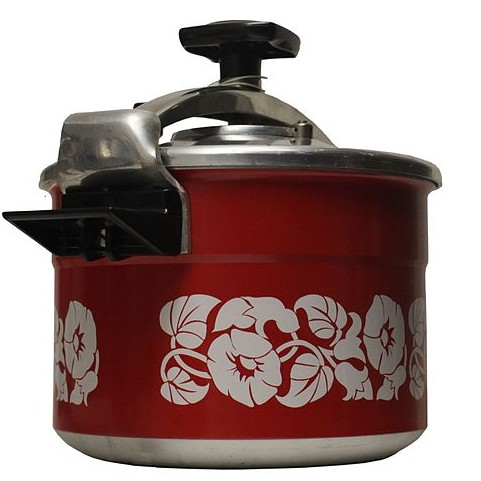
\includegraphics[width=8cm]{images/exercice_super_cocotte}
		\end{center}
		\supercaption{Autocuiseur ou cuiseur à pression, couramment appelé \textit{«~cocotte-minute~»} en France.}{\wcfile{Super_Cocotte_decor_SEB-MGR_Lyon-IMG_9918.jpg}{Photo} \ccbysa par \wcu{rama}}
		\label{fig_cocotte}
	\end{figure}


\subsubsection{Un premier moteur à vapeur}

	Un/e ingénieur/e expérimente avec de la vapeur d’eau, dans l’idée de mettre au point un petit moteur très simple (\cref{fig_moteurvapeursimple})
	
	Il/elle insère \SI{2}{\liter} d’eau liquide à~\SI{20}{\degreeCelsius} dans un grand cylindre. L’eau est comprimée à~\SI{2}{\bar} par un piston.
	
	Il/elle chauffe l’eau, et le piston se déplace en maintenant la pression constante, jusqu’à ce que le volume ait atteint~\SI{300}{\liter}.
	
	\begin{enumerate}
		\item Tracez qualitativement l’évolution suivie par le fluide sur un diagramme pression-volume ou température-volume.
		\item Quel a été le travail effectué ?
		\item Combien de chaleur a-t-il fallu apporter ?
		\item Quels seraient les transferts de travail et de chaleur si la détente était poursuivie jusqu’à~\SI{4500}{\liter} ?
	\end{enumerate}

	\begin{figure}[htp] %handmade
		\begin{center}
			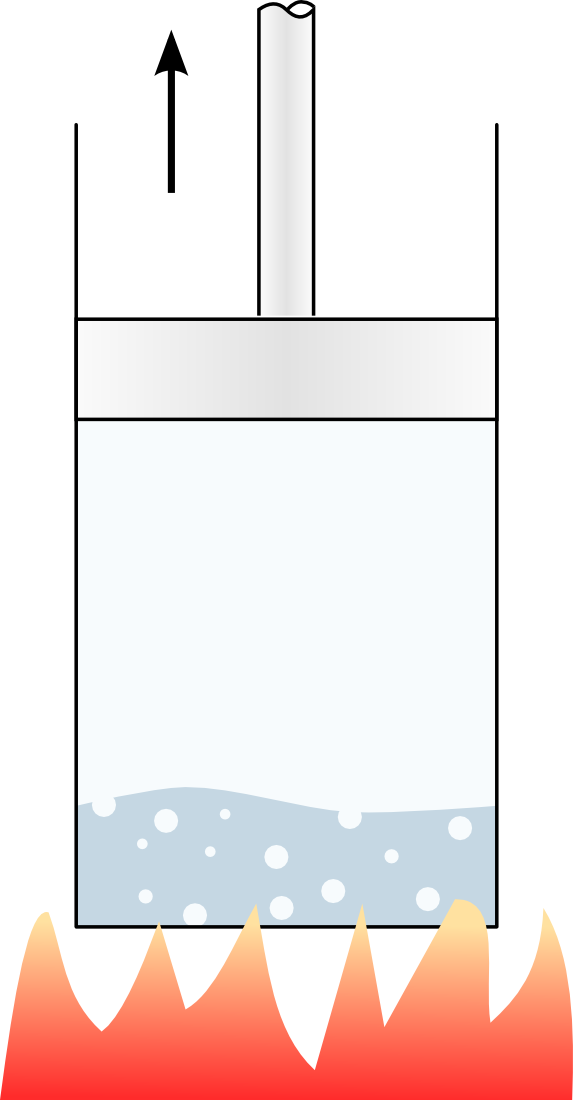
\includegraphics[width=4cm]{images/exercice_moteur_simple.png}
		\end{center}
		\caption{Un concept très simple de moteur à vapeur}
		\label{fig_moteurvapeursimple}
	\end{figure}

\subsubsection{Pompage d’eau}

	Une pompe à eau est installée pour prélever de l’eau à~\SI{5}{\degreeCelsius} située dans un réservoir en contrebas (\cref{fig_pompage}). 
	
	\begin{enumerate}
		\item Jusqu’à quelle hauteur peut-on effectuer le pompage ?	
		\item Comment pourrait-on procéder pour pomper l’eau à plus grande hauteur ?
	\end{enumerate}

	\begin{figure}[htp] %handmade
		\begin{center}
			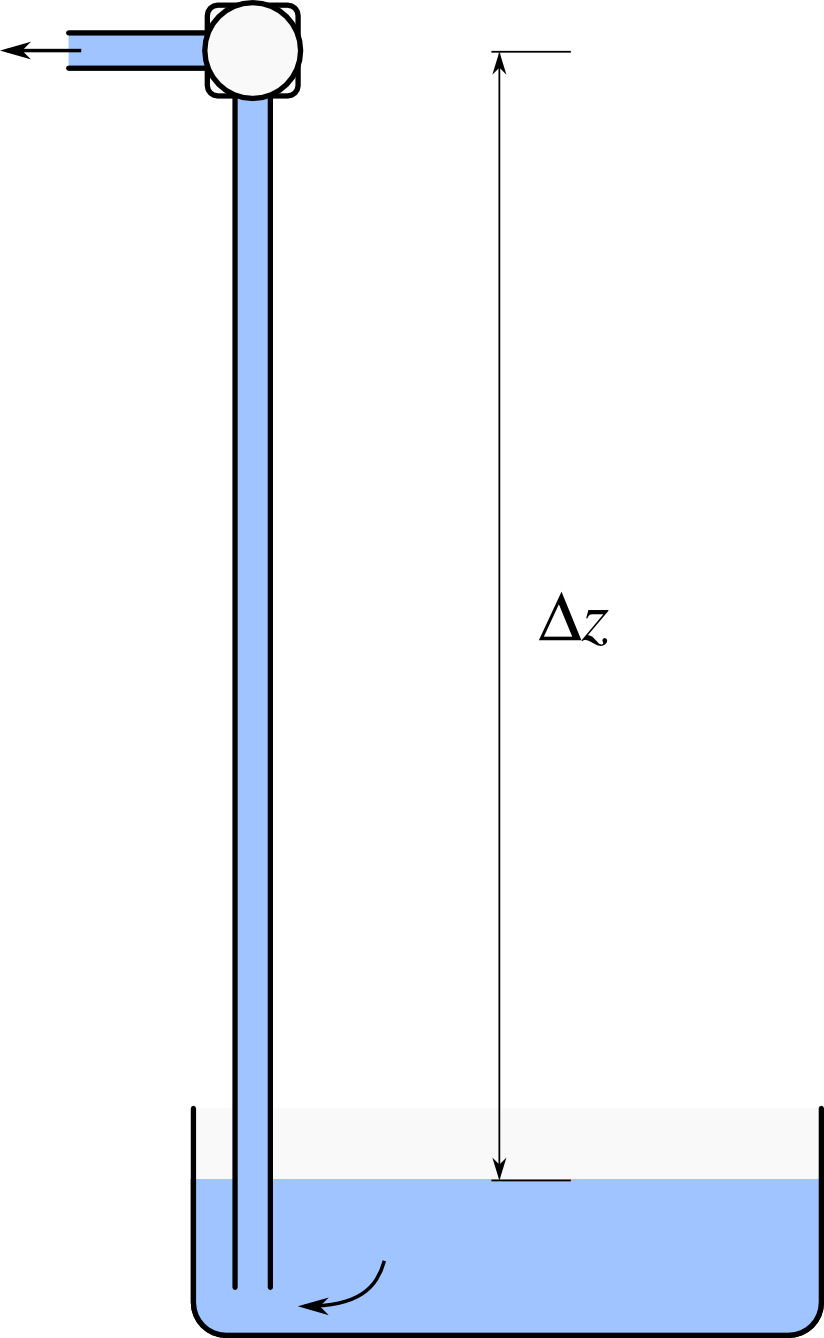
\includegraphics[width=5cm]{images/exercice_pompe_eau.png}
		\end{center}
		\supercaption{Pompage d’un réservoir d’eau situé en contrebas. La première observation de la limite de hauteur calculée dans cet exercice est faite en 1630 par \wf{Giovanni Battista Baliani}.}{\cczero}
		\label{fig_pompage}
	\end{figure}



\subsubsection{Turbine à vapeur sur installation légère}

	Une entreprise développe une petite centrale à vapeur pouvant être embarquée dans un container de taille standard. Une fois reliée à une chaudière externe, elle est capable de convertir de la chaleur provenant de combustibles peu raffinés (comme le bois, le papier ou le charbon) en électricité, avec une efficacité intéressante.
	
	Au sein de cette centrale, la turbine est adiabatique et admet \SI{5}{\tonne\per\hour} de vapeur à~\SI{90}{\bar} et~\SI{510}{\degreeCelsius} en provenance de la chaudière. La pression de sortie est (à peine supérieure à) la pression atmosphérique (nous prendrons \SI{1}{\bar}). Un/e ingénieur prévoit\footnote{Nous pourrons aussi faire cela après le \courshuit.} que l’énergie interne spécifique de la vapeur sera alors de~\SI{2676,6}{\kilo\joule\per\kilogram}.
	
	La turbine est mécaniquement connectée à une génératrice de courant d’efficacité~\SI{85}{\percent}.
	
	\begin{enumerate}
		\item Quelle est la puissance électrique dégagée par la génératrice ?
	\end{enumerate}
	
	À l’autre extrémité du container, une pompe électrique (seul autre élément mécanique de l’installation) récupère l’eau condensée à l’état de liquide saturé (\SI{1}{\bar}) et augmente à nouveau sa pression jusqu’à~\SI{90}{\bar} pour alimenter la chaudière. On considère que lors du pompage, le volume spécifique de l’eau varie de façon négligeable, et que la compression est réversible.
	
	\begin{enumerate}
	\shift{1}
		\item Quelle puissance électrique est prélevée pour alimenter la pompe ?
	\end{enumerate}
	



\subsubsection{Le baril écrasé}

	Pour effectuer une démonstration de physique, un groupe d’étudiants porte de l’eau  dans un ancien baril de pétrole (contenance \SI{208}{\liter}, hauteur \SI{88}{\centi\metre}) à ébullition, à pression ambiante.
	
	Le baril est retiré de la source de chaleur et est fermé de façon hermétique. Le but de l’expérience est bien sûr de le voir se contracter suite au changement d’état de l’eau à l’intérieur.

	\begin{enumerate}
		\item Quelle dépression peut-on atteindre à l’intérieur du baril en le laissant se refroidir ? 
		\item Quelle serait alors la force verticale s’appliquant sur la paroi supérieure du baril ?
	\end{enumerate}
	
	\textit{Et pour ceux qui souhaitent poursuivre :}
		
	\begin{enumerate}
	\shift{2}
		\item Il reste \SI{5}{\liter} de liquide au fond du baril à la fermeture du bouchon. Quel est le titre de la vapeur ?
		\item Quelle masse de vapeur s’est condensée pendant le refroidissement ?
		\item Combien a-t-il fallu retirer de chaleur pour atteindre la dépression finale ?
	\end{enumerate}

\clearpage
\subsubsection{Moteur Newcomen}

	À leur époque, autour de 1720, les moteurs Newcomen (\cref{fig_newcomen}) étaient à la pointe de la technologie. On insérait dans un grand cylindre (hauteur \SI{1}{\metre}, diamètre \SI{1.5}{\metre}) de la vapeur à peine surchauffée (\SI{1}{\bar}, \SI{250}{\degreeCelsius}).
	
	Puis, on refroidissait cette vapeur (en faisant rentrer de l’eau liquide à pression et température atmosphériques), en maintenant la pression interne à~\SI{0,1}{\bar}. Le piston redescendait ainsi en fournissant du travail.
	
	\begin{enumerate}
		\item Tracez l’évolution suivie par l’eau sur un diagramme pression-volume ou température-volume, en y indiquant la courbe de saturation.
		\item Quelle quantité de travail est dégagée par le moteur pendant la descente du piston ?
		\item Avant de pouvoir effectuer la descente, quelle quantité de chaleur a-t-il fallu pour amener l’eau dans le cylindre (l’eau disponible étant à~\SI{1}{\bar}, \SI{10}{\degreeCelsius}) ?
		\item Quel est ainsi le rendement du moteur, si l’on néglige toutes les autres pertes de chaleur ?
	\end{enumerate}

	\begin{figure}[htp] %handmade
		\begin{center}
			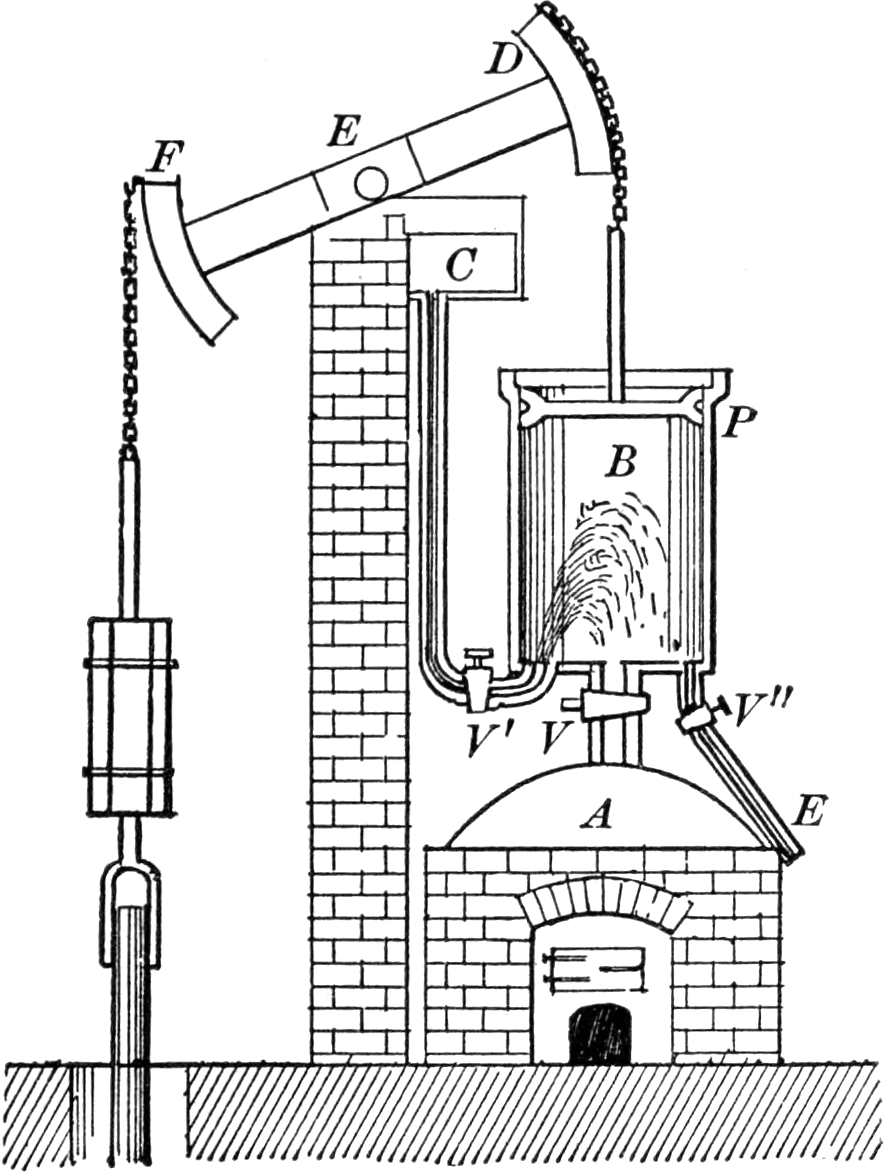
\includegraphics[width=9cm]{images/Newcomen6325.png}
		\end{center}
		\supercaption{L’ingénieux moteur atmosphérique de Newcomen, premier véritable succès de la motorisation vapeur.}{\wcfile{Newcomen6325.png}{schéma} \pd (pub. 1913 in Practical physics for secondary schools. Fundamental principles and applications to daily life) par Newton Henry Black et Harvey Nathaniel Davis}
		\label{fig_moteur_newcomen}
	\end{figure}



\subsubsection{Condenseur de centrale à vapeur}

	Dans une centrale électrique de grande puissance, le condenseur est en charge de récupérer l’eau à la sortie des turbines, et de lui retirer de l’énergie pour qu’elle puisse retourner à l’état liquide et ré-intégrer le circuit pompes $\to$ chaudières $\to$ turbines. L’eau du circuit (\SI{180}{\tonne\per\hour}) arrive à~\SI{0,5}{\bar} avec un volume spécifique de~\SI{3,1247}{\metre\cubed\per\kilogram}; elle doit repartir à la même pression, à l’état de liquide saturé.
	
	Pour extraire de la chaleur à l’eau de la centrale, les condenseurs utilisent un circuit d’eau secondaire provenant directement d’une rivière. On y prélève de l’eau à~\SI{10}{\degreeCelsius}.
	
	Pour réduire l’impact écologique de la centrale, on souhaite rejeter l’eau secondaire dans la rivière à une température égale ou inférieure à~\SI{35}{\degreeCelsius}.
	
	\begin{enumerate}
		\item Quel débit d’eau secondaire doit-on prélever en rivière ?
		\item Pour limiter les rejets de chaleur en rivière, où (et comment) rejette-t-on aussi la chaleur du condenseur ?
	\end{enumerate}
	

\subsubsection{Catapulte de porte-avions}

	Une catapulte à avions est montée sur un navire militaire (\cref{fig_catapultes}). Elle est constituée d’un réservoir de vapeur connecté à un long cylindre, dans lequel glisse un piston entraînant l’avion au décollage.
	
	Au début du catapultage, la vapeur est à~\SI{140}{\bar} et~\SI{700}{\degreeCelsius}. Après une brève course de~\SI{50}{\metre}, l’avion a quitté le pont et la vapeur est à~\SI{4}{\bar} et~\SI{410}{\degreeCelsius}.
	
	\begin{enumerate}
		\item Quelle énergie la catapulte a-t-elle fourni à l’avion par kilo de vapeur ?
		\item Quelles doivent être le diamètre du piston, et la masse totale de vapeur, pour que la poussée fournie à l’avion soit toujours supérieure à~\SI{2,5}{\tonne} ?
		\item \textit{(question à laquelle nous ne savons pas encore répondre)} Quelle est la quantité \emph{maximale} d’énergie que la catapulte aurait pu fournir à l’avion en laissant la vapeur se détendre ?
	\end{enumerate}
	
	\begin{figure}
		\begin{center}
			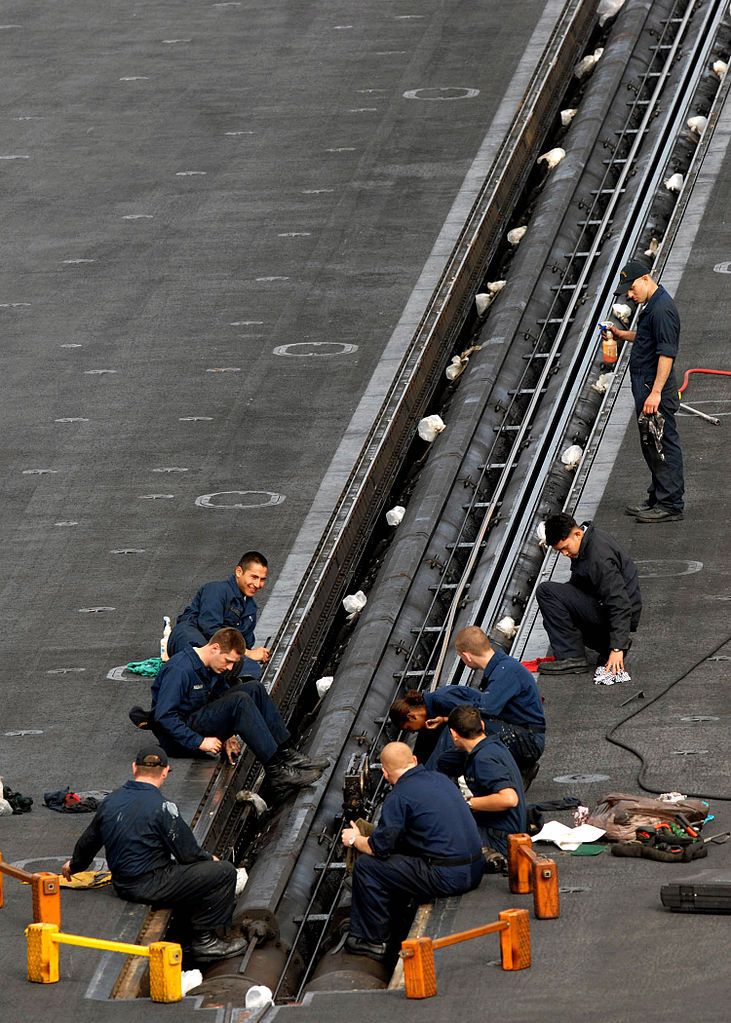
\includegraphics[height=0.44\textwidth]{images/catapulte_vapeur_1.jpg}
			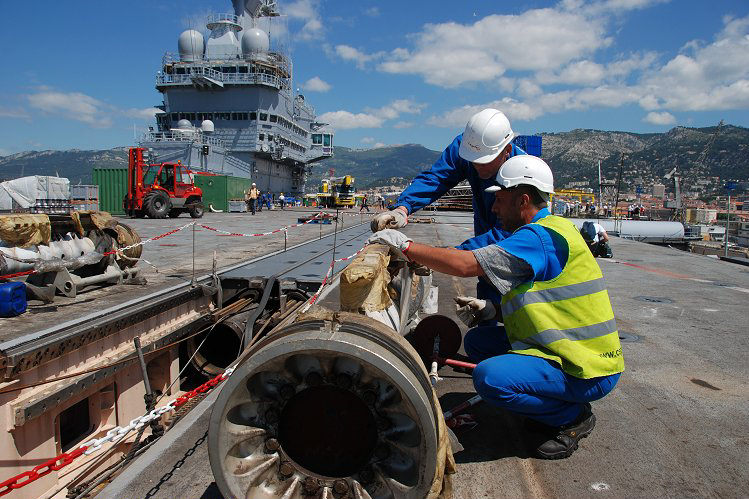
\includegraphics[height=0.44\textwidth]{images/catapulte_vapeur_2.jpg}
		\end{center}
		\supercaption{Cylindre d’une catapulte à vapeur du USS Abraham Lincoln (gauche), et piston d’une catapulte à vapeur du Charles de Gaulle (droite).}{\wcfile{Catapulte CVN72 071117-N-9898L-006.jpg}{Photo 1} \pd par Geoffrey Lewis, U.S. Navy\\
						\wcfile{French aircraft carrier Charles de Gaulle - catapult maintenance 2008.jpg}{Photo 2} \ccbysa par Jean-Michel Roche, Netmarine.net}
		\label{fig_catapultes}
	\end{figure}

\subsubsection{Turbine de centrale nucléaire}

	Dans une centrale nucléaire, la génératrice d’électricité est entraînée par une turbine à vapeur (\cref{fig_centrale_balakovo}).\\
	La majorité de la vapeur (chauffée par le réacteur nucléaire) traverse l’entièreté de la turbine. Toutefois, au milieu de la turbine, on procède à un prélèvement de vapeur. Il permet, d’une part, de réchauffer l’eau d’une autre partie du circuit, et d’autre part, de contrôler précisément le débit de masse en circulation. La turbine est ainsi divisée en deux sections en série. Le débit total à l’entrée est de~\SI{317}{\tonne\per\hour} de vapeur.
	
	On mesure les propriétés de vapeur suivantes :
	
	\begin{description}
		\item Entrée : 		\SI{120}{\bar} ; 	\SI{565}{\degreeCelsius}
		\item Prélèvement : 	\SI{10}{\bar} ; 	\SI{250}{\degreeCelsius} ;	\SI{1,2}{\kilogram\per\second}
		\item Sortie : 		\SI{1}{\bar} ;		\SI{115}{\degreeCelsius}
	\end{description}

	Quelle est la puissance mécanique fournie par la turbine ?

	\begin{figure}
		\begin{center}
			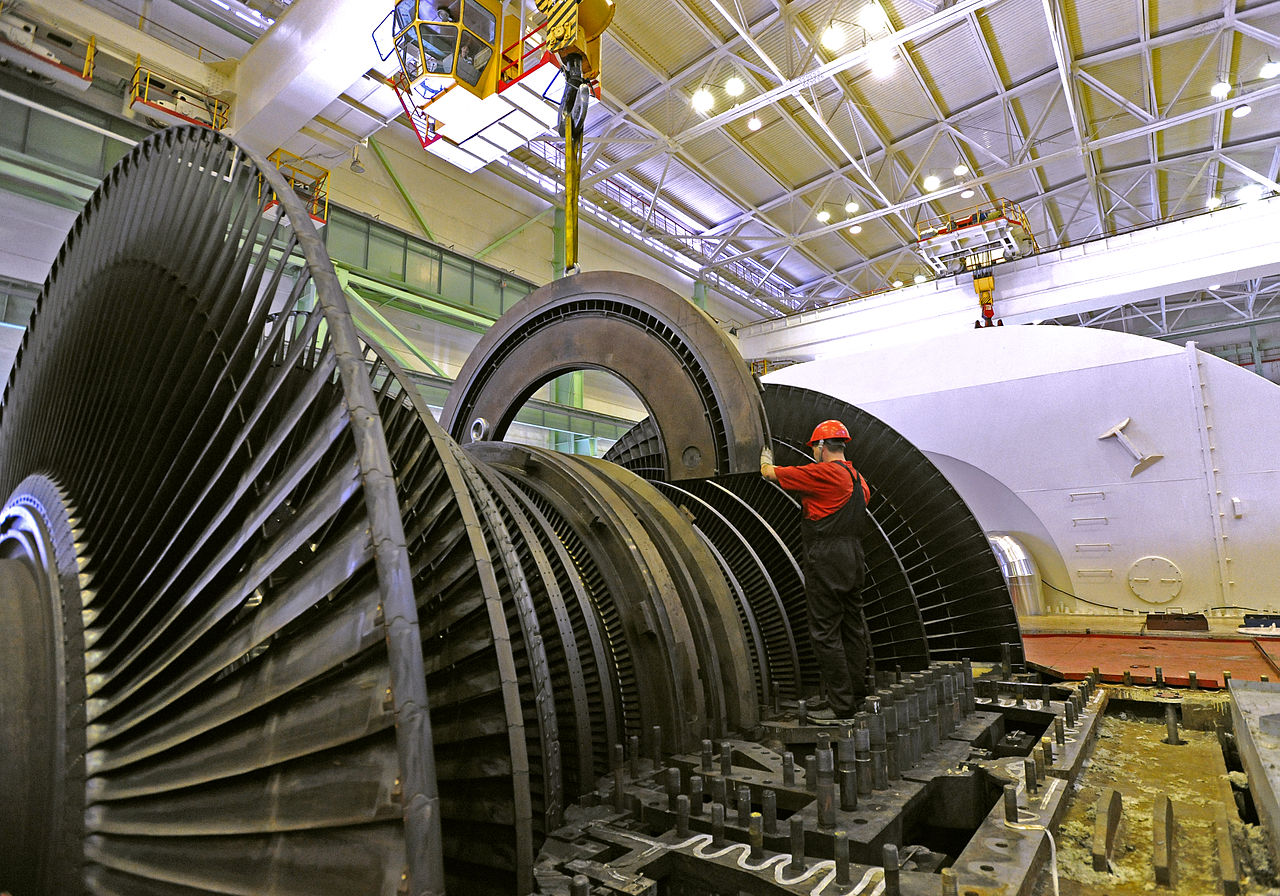
\includegraphics[height=0.33\textwidth]{images/exercice_turbine_centrale2.jpg}
			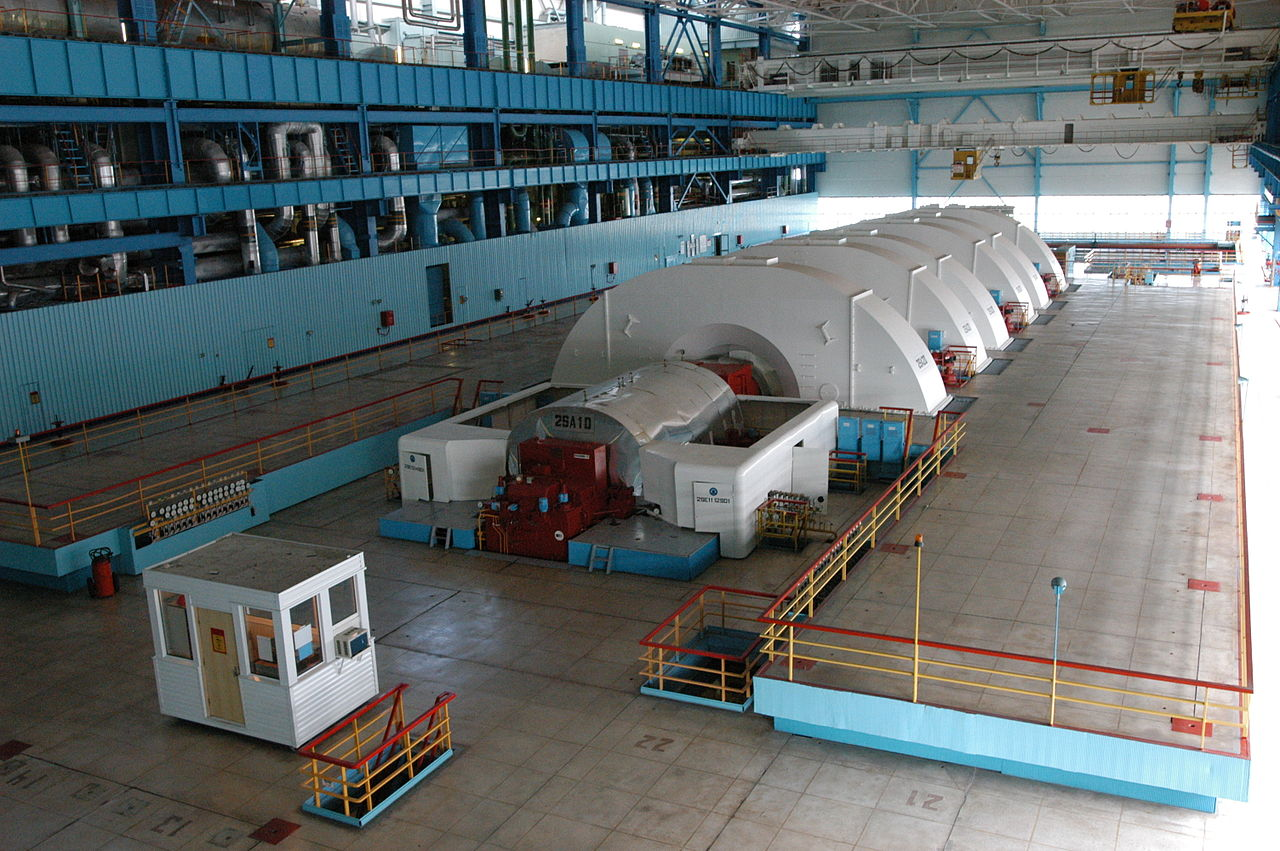
\includegraphics[height=0.33\textwidth]{images/exercice_turbine_centrale1.jpg}
		\end{center}
		\supercaption{Une des turbines de la centrale nucléaire russe de Balakovo (puissance approx.~\SI{1}{\giga\watt}), en maintenance (haut) et en installation (bas).}{\wcfile{BalakovoNPP_turb.JPG}{photo 1} et \wcfile{BalNPP_m_st2.jpg}{2} \ccbysa The Centre of the Public Information Balakovo NPP}
		\label{fig_centrale_balakovo}
	\end{figure}

\exercisesolutionpage
\subsubsection*{Résultats}
	\linktosolutionsblurb

	\begin{description}
		\item [5.1] \SI{0,67}{\bar} ; \SI{56,8}{\degreeCelsius} (berk!)
		\item [5.2] \num{0,29}\euro{} (en \SI{1}{\hour} et~\SI{21}{\minute})
		\item [5.4] $\dot{Q}_{1 \to 2} = \SI{+8,59}{\mega\watt}$, $\dot{W}_{1 \to 2} = \SI{0}{\watt}$
		\item [5.5] 1) \SI{121,37}{\degreeCelsius} (ne pas oublier la pression atmosphérique)
		\item [5.6] \tab 2) ${W}_{2 \to 4} = \SI{-59,6}{\kilo\joule}$ 
						\tab 3) ${Q}_{1 \to 2} = \SI{+1585,2}{\kilo\joule}$ (on a $x_4 = \num{0,1697}$) 
						\tab 4) ${W}_{2 \to 5} = \SI{-899,6}{\kilo\joule}$ et ${Q}_{2 \to 5} = \SI{+7694,3}{\kilo\joule}$
		\item [5.7] $\Delta p_\text{ébullition} = \SI{9,9127e4}{\pascal}$, $\Delta z_\text{ébullition} = \SI{10,1}{\metre}$
		\item [5.8] $\dot{W}_\text{électrique} = \SI{-605,8}{\kilo\watt}$ ; $\dot{W}_\text{pompe} = \SI{+12,9}{\kilo\watt}$
		\item [5.9] \tab 1) Si on atteint $T_\text{final} = \SI{20}{\degreeCelsius}$, $\Delta p_\text{max} = \SI{-9,575e4}{\pascal}$
						\tab 2) \SI{22,6}{\kilo\newton} (le baril sera bien sûr écrasé avant)
						\tab 4)  $x_1 = \num{0,02408}$, $x_2 = \num{7,328e-4}$ ; ${Q}_{1 \to 2} = \SI{-1,878}{\mega\joule}$
		\item [5.10] \tab 2)${W}_\text{piston $\to$ arbre} = \SI{-159}{\kilo\joule}$
						\tab 3)  ${Q}_\text{réchauff} = \SI{+2185}{\kilo\joule}$
						\tab 4) $\eta = \SI{7,28}{\percent}$.
		\item [5.11] $\dot{m}_\text{secondaire} = \SI{1062,4}{\kilogram\per\second}$
		\item [5.12] \tab 1) ${w}_{1 \to 2} = \SI{-433,1}{\kilo\joule\per\kilogram}$
						\tab 2) $D_\text{min.} = \SI{32,26}{\centi\metre}$, $m = \SI{5,243}{\kilogram}$ (attention à tenir compte de la pression atmosphérique)
		\item [5.13] $\dot{W}_{1 \to 3} = \SI{-71}{\mega\watt}$
	\end{description}
